\documentclass[11pt, oneside]{article} 
\usepackage{geometry}
\geometry{letterpaper} 
\usepackage{graphicx}
	
\usepackage{amssymb}
\usepackage{amsmath}
\usepackage{parskip}
\usepackage{color}
\usepackage{hyperref}

\graphicspath{{/Users/telliott_admin/Dropbox/Tex/png/}}
% \begin{center} 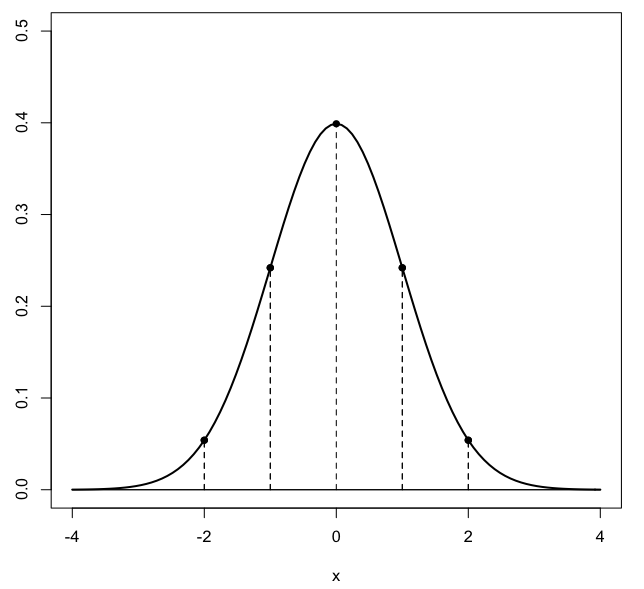
\includegraphics [scale=0.4] {gauss3.png} \end{center}

\title{Analytic geometry}
\date{}

\begin{document}
\maketitle
\Large

It is difficult today to put ourselves in the places of those who tried to reason about mathematics through the ages.  For example, the Greeks lacked algebra, and although the Romans worked with numbers they lacked decimal notation.  The concept of $0$ came much later (from India), and even in the Middle Ages there was as yet no such thing as the equals sign $=$, which dates from 1557.

\url{https://en.wikipedia.org/wiki/Table_of_mathematical_symbols_by_introduction_date}

The invention of analytic geometry is often ascribed solely to Descartes, but Fermat also had a big role.  There are two fundamental ideas.
\begin{center} 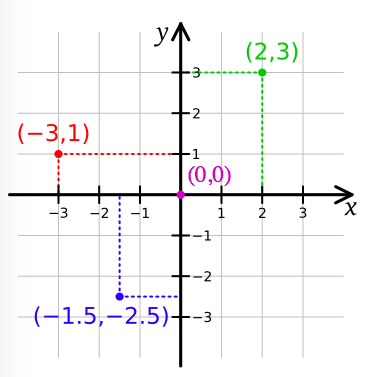
\includegraphics [scale=0.45] {coordinates.png} \end{center}

The first is to orient two number lines on a piece of paper, at right angles, and then consider pairs of numbers $(x,y)$ in the 2D plane.  Such pairs or tuples are called points.

Descartes published this idea in 1637.  The presentation would be difficult to recognize as our current system, but the germ is there:  axes where the position of a variable could be marked.  Only the positive numbers would be shown, and the axes not necessarily perpendicular.  As to the proofs, here is wikipedia on the subject:

\begin{quote}
His exposition style was far from clear, the material was not arranged in a systematic manner and he generally only gave indications of proofs, leaving many of the details to the reader.  His attitude toward writing is indicated by statements such as "I did not undertake to say everything," or "It already wearies me to write so much about it," that occur frequently. In conclusion, Descartes justifies his omissions and obscurities with the remark that much was deliberately omitted "in order to give others the pleasure of discovering [it] for themselves."
\end{quote}

The second idea of analytic geometry is to plot all the points that satisfy some mathematic relationship between $x$ and $y$, for example the parabola $y=x^2$.  

To do this, pick a few values of $x$ and calculate the corresponding values of $y$.  For example:  $(0,0), (\pm 1,1), (\pm 2, 4), \dots$.  Plot these points, and then finally, sketch the graph of the curve, without actually trying to plot \emph{all} of the individual points (of which there is an infinite number).  We make the assumption here that the function being plotted is continuous, so that the sketch of a curve between two points that are close enough together will be fairly smooth and for $x$-values close to the plotted $x$, have corresponding $y$-values not too different from the plotted $y$.

\subsection*{formulas for a line}

Suppose we pick two points $(x_1,y_1)$ and $(x_2,y_2)$, plot them on a graph, and then draw the line that connects them.  Recall Euclid's first two postulates:

$\circ$  A straight line segment can be drawn joining any two points.

$\circ$   Any straight line segment can be extended indefinitely in a straight line.
 
Now we want to derive an equation that describes (is valid for) all the points or pairs of values $(x,y)$ on this line.  A general approach is to say that the line has some slope $m$, which is defined as the rate of change of $y$, called $\Delta y$, divided by the rate of change of $x$:

\[ m = \frac{\Delta y}{\Delta x} = \frac{y_2 - y_1}{x_2 - x_1} \]

This is the \emph{point-slope equation}.

The value of $m$ might be zero, for a horizontal line, where all the values of $y$ are the same.  Or it might be undefined, for a vertical line, where all the values of $x$ are identical.  

In most cases, however, $m \ne 0$ and $m \in (-\infty, \infty)$.  That is, $|m|$ is not infinite but also non-zero.

Except in the case of the vertical line, we can write
\[ y = mx + b \]

for any two points $x$ and $y$ on a given line.  $b$ is called the $y$-intercept, it is the value of $y$ obtained when $x = 0$.  This is the \emph{slope-intercept equation} of the line.

Notice that the equation of a line is not determined just by the slope.  One can draw a whole family of parallel lines with the same slope and different $y$-intercepts.  For example here are three lines $y = 2x + b$ for $b = \{ 0, 1, 2 \}$.

\begin{center} 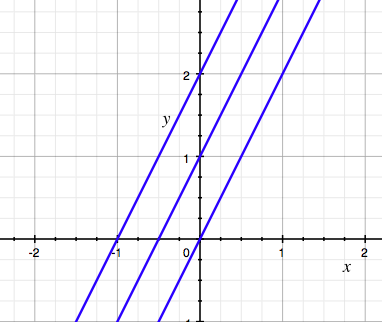
\includegraphics [scale=0.4] {line_family.png} \end{center}

The value of $x$ corresponding to $y = 0$ is the $x$ intercept
\[ x = -\frac{b}{m} \]

The first equation is easily derived from the second.  Plugging in specific values of $x$ and $y$ we have
\[ y_1 = mx_1 + b \]
\[ y_2 = mx_2 + b \]
Subtracting
\[ y_2 - y_1 = m(x_2 - x_1) \]
which rearranges to give the desired result.

\subsection*{formula for a circle}

A circle can be defined as all the points at the same distance from a central point, let us label that point $(h,k)$.  The distance from the points to the center is the radius, denoted $r$.

Using the Pythagorean theorem, we can calculate the square of the distance from the origin as
\[ r^2 = (x - h)^2 + (y - k)^2 \]

The simplest circles are those whose central point is the origin of the coordinate system.  In that case the equation  simplifies to 
\[ r^2 = x^2 + y^2 \]
Usually, we know the value of $r$ and we want to write an equation for $y$ in terms of $x$.  Then
\[ y^2 = r^2 - x^2 \]
\[ y = \sqrt{r^2 - x^2} \]

\subsection*{example}

Here is a moderately complicated example we will see much later in the book (\hyperref[sec:quad]{\textbf{here}}).

\begin{center} 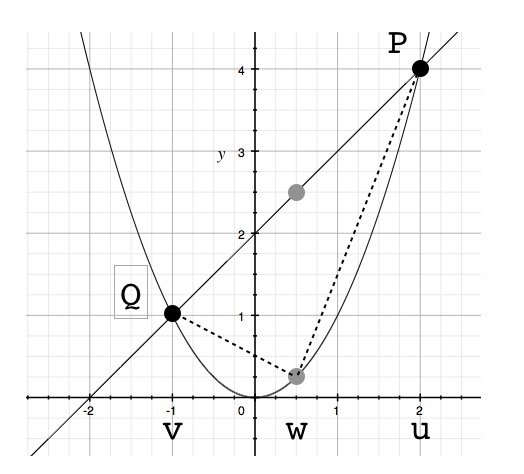
\includegraphics [scale=0.4] {para_tri2.png} \end{center}

It shows the two axes (horizontal and vertical lines with distances marked), and four points plotted plus a line, two line segments, and a parabola.  We can also "read" other points off the graph, such as the vertex of the parabola $(0,0)$, or the intersections of the line with the axes at $(-2,0)$ and $(0,2)$.

It is assumed you've studied analytic geometry before, so we won't say much more now than what is in this chapter.

Much of a standard course in analytic geometry is concerned with the conic sections:  circle, ellipse, parabola and hyperbola.  Those are all wonderful topics, but we'll wait to explore them in detail in later chapters, where we can use a bit of calculus and also linear algebra.  

For now, let's continue with trigonometry before getting back to the main subject.

\end{document}